\subsection{Common-Emitter Amplifier with Fixed Bias Circuit}
Assemble the circuit shown in the following figure.
\begin{figure}[h]
    \centering
    \includegraphics[width = 0.5\textwidth]{Imagenes/Imagenes_Juan/Amplificador en Emisor Común en Circuito.PNG}
    \caption{Common-Emitter Amplifier with Fixed Bias Circuit}
    \label{circuit1}
\end{figure}

Without turning on the generator, measure the operating point.

\begin{center}
    Q( 5.81 V, 5.92 mA).
\end{center}


Then, apply a sinusoidal input signal of 50 mV at a frequency of 1 kHz.
On the oscilloscope, observe the input voltage signal on channel 1 and the output voltage signal on channel 
2. Compare the phase (note the inversion of the output signal with respect to the input), determine the 
gain, and plot the obtained waveforms.

\begin{center}
    IMAGEN OSCILOSCOPIO
\end{center}

\begin{table}[H]
\centering
\caption{Resultados del experimento}
\label{tab:resultados}
\begin{tabular}{lccc} % 4 columnas: primera izquierda, otras centradas
\toprule
 & Input & Output & Gain \\ 
\midrule
Practical   & 120 mV & 1.84 V & 1.7 V\\ 
Theoretical & 100 mV & 5.28 V & 5.18 V\\ 
Simulated   & 100 mV & 6.8 V & 6.7 V \\ 
\bottomrule
\end{tabular}
\end{table}

\newpage

\subsection{Common-Emitter Amplifier with Emitter-Stabilized Bias Circuit}

Assemble the circuit shown in the following figure.
\begin{figure}[h]
    \centering
    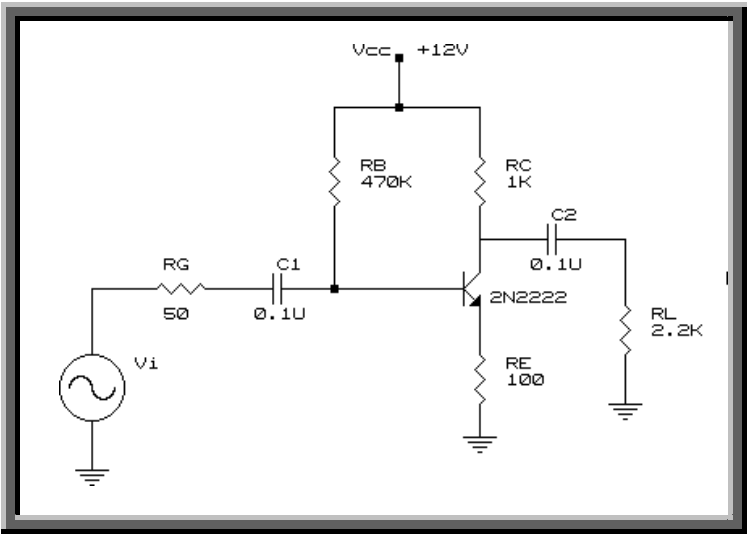
\includegraphics[width = 0.5\textwidth]{Imagenes/Imagenes_Juan/Common-Emitter Amplifier with Emitter-Stabilized Bias Circuit.PNG}
    \caption{Common-Emitter Amplifier with Emitter-Stabilized Bias Circuit}
    \label{circuit2}
\end{figure}

Without turning on the generator, measure the operating point.

\begin{center}
    Q( 5.65 V, 5.49 mA).
\end{center}

Then, apply a sinusoidal input signal of 50 mV at a frequency of 1 kHz.
On the oscilloscope, observe the input voltage signal on channel 1 and the output voltage signal on channel 
2. Compare the phase (note the inversion of the output signal with respect to the input), determine the 
gain, and plot the obtained waveforms.

\begin{figure}[h]
    \centering
    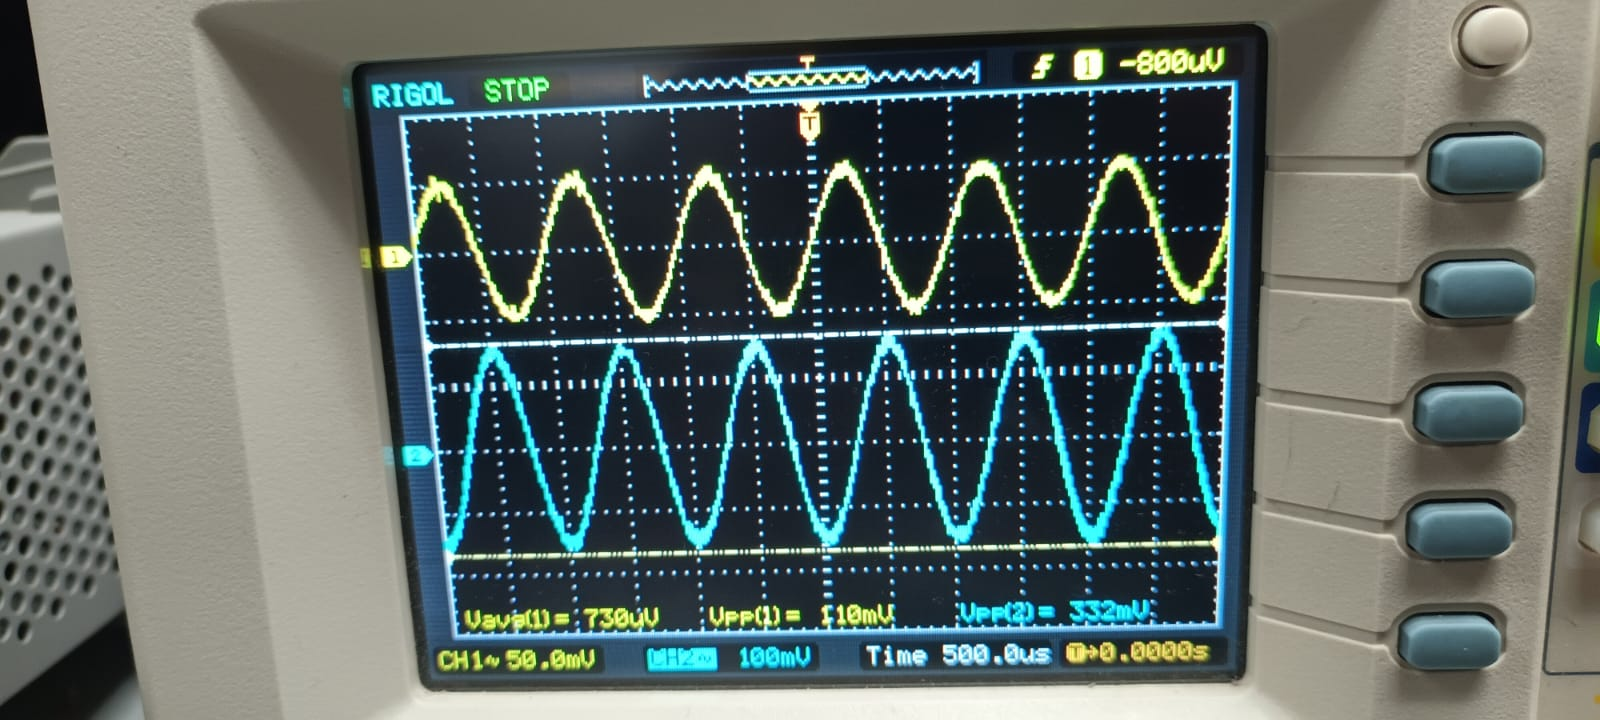
\includegraphics[width = 0.9\textwidth]{Imagenes/Imagenes_Juan/Osciloscopio Circuito 2.jpg}
    \caption{Common-Emitter Amplifier with Emitter-Stabilized Bias Circuit on the oscilloscope}
    \label{circuit2Osciloscopio}
\end{figure}

\begin{table}[H]
\centering
\caption{Resultados del experimento}
\label{tab:resultados2}
\begin{tabular}{lccc} % 4 columnas: primera izquierda, otras centradas
\toprule
 & Input & Output & Gain \\ 
\midrule
Practical   & 110 mV & 332 mV & 222 mV\\ 
Theoretical &  &  & \\ 
Simulated   &  &  &  \\ 
\bottomrule
\end{tabular}
\end{table}




